%~~~~~~ Packages ~~~~~~
\RequirePackage{fix-cm}
\documentclass[smallextended]{svjour3}       
\smartqed                                    
\usepackage{graphicx}
\usepackage{mathtools}
\usepackage{amssymb}
\usepackage{amsmath}
\usepackage{tabularx}
\usepackage{color}
\usepackage{mdframed}
\usepackage{tikz}                        
\usepackage{wrapfig}
\usepackage{indentfirst}
\usepackage{mathptmx}                             
\usepackage{latexsym}

%~~~~~~ Commands ~~~~~~ 
%D.E.
\newcommand{\od}[3][]{\ensuremath{\frac{\mathrm{d}^{#1} {#2}}{\mathrm{d}{#3}^{#1}}}}
%TODO
\newcommand{\todo}[1]{{\huge\color{red}TODO {#1}}}
%Team Notice
\newcommand{\Notice}[1]{{\huge\color{pink}NOTICE {#1}}}
%Question
\newcommand{\Query}[1]{{\huge\color{green}Question: {#1}}}
%Notes
\newcommand{\TwoNote}[4]{$$\text{Note:}\quad\left\{\begin{aligned} {#1} \text{\quad #2} \\
{#3} \text{\quad #4} \\ \end{aligned}\right\}.$$}
%OneNote
\newcommand{\OneNote}[2]{$$\text{Note:}\quad\left\{\begin{aligned} {#1} \text{\quad #2} \end{aligned}\right\}.$$}
%ZeroNote
\newcommand{\ZeroNote}[1]{$$\text{Note:}\quad\left\{\begin{aligned} {#1} \end{aligned}\right\}.$$}
%TextBox
\renewcommand{\thefigure}{\Roman{figure}}
\DeclareMathOperator*{\argmax}{arg\,max}
\definecolor{silver}{rgb}{0.95,0.95,0.95}

%~~~~~~ Journal Name ~~~~~~
\journalname{Journal of Mathematical Biology}
%~~~~~ Begin Document ~~~~~~
\begin{document}
%~~~~~~ Title & Subtitle ~~~~~~
\title{Mathematical Model of the Enzymatic Production, Transport, and Use of Dopamine }
\subtitle{in the Renal and Gastrointestinal Systems; Circulatory System; and the Central Nervous System}
%~~~~~~ Authors ~~~~~~
\author{Wolesensky B. \and
        Frisby L. \and
        Smith C. \and
        Wheeler G.\and
        Wolesensky  D.
}                                
\institute{B. Wolesensky \at                                           
              University of Texas at Austin \\
              Tel.: +123-45-678910\\
              Fax: +123-45-678910\\
              \email{fauthor@example.com}
           \and
           L. Frisby \at                                               
              2501 Pearl St. Unit 103
              \and                          
          C. Smith \at                                                 
              University of Texas at Austin \\
              \and               
          G. Wheeler \at                                               
              Gerrit's Info 
              \and 
          D. Wolesensky \at                                            
              Danielle's Info     
}
\date{Received: July 2016 / Accepted: date}
%~~~~~~ABSTRACT~~~~~~
\maketitle
\begin{abstract} 			
\Notice{Please Don't make Changes to this Version. Building new Outline. Will send link as soon as possible}  Lack of dopamine is a known cause of Parkinson's as well as other illnesses.  Though it is believed that Parkinson's Disease is due to a lack of dopamine in the Nigrostriatal Dopaminergic pathway, current medications and treatments which directly treat the lack of dopamine within the pathways are ineffective at best.  Our model introduces a theory to explain the lack of dopamine within the Nigrostriatal Dopaminergic pathway in Parkinson's patients. Dopamine is synthesized from its mirror image, L-DOPA which is created both within the digestive system and kidneys and transported via the circulatory system through the blood brain barrier to the Dopaminergic Pathways where it is transported directly to the neuron via the transport protein AADC before being synthesized into dopamine.  It has long been known that L-DOPA is processed en-masse via the kidneys, specifically within the Proximal Tubule Cells.  However, the method by which L-DOPA is stored and transported within these Proximal Tubule Cells is poorly understood and no mechanistic model currently exists.  The following provides a comprehensive mechanistic model for the synthesis, transport and uptake of dopamine within the body.  Additionally our simulations show an over production of dopamine in the kidneys leaves little L-DOPA for synthesis into dopamine within the Nigrostriatal Pathway. Wrap this up at the end... Include keywords, PACS and mathematical subject classification numbers as needed.
  
\Query{PACS? and mathematical subject classification numbers?} %Question

\keywords{Nigrostriatal Pathway \and L-DOPA \and Dopaminergic Pathway \and Parkinson's \and Michaelis Menten \and Dopamine \and Tyrosine \and Enzyme \and Complex \and Substrate \and Proximal Tubule Cell \and Explanatory \and Mechanistic \and Gastrointestinal \and Circulatory \and Kidney \and Brain \and VTA \and ODE \and IVP \and etc.}
\end{abstract}

%~~~~~~ SECTION 1 ~~~~~
\section{Introduction}
\label{sec:1}
\todo{needs editing}

There lacks a mechanistic model of Dopamine that follows the pathway from start to finish. The Dopamine cycle itself is difficult to understand and current research is focusing on gaining a deeper understanding of what goes on (CITATION NEEDED). A mechanistic model would help to tell the story and allow for manipulations, changes, and simulations along each step in order to test hypotheses, drug treatment options, and simply gain a better overall understanding of what Dopamine is doing before it interacts with our brain. A good model would allow the mathematics to drive science as opposed to science driving applied mathematics (Bill paraphrase, not sure how that sounds...).Dopamine has been difficult for researchers to fully understand despite over 50 years of research on the topic. Major progress has been made but it seems the more that is discovered about Dopamine the more important Dopamine becomes. Dopamine is now known to effect mood, motor function, cognition, addiction, and reward \cite{Ref34}. \\
%
\indent Dopamine affects people at every moment of every day, it is no wonder why researchers have worked so hard on understanding it. This model does not attempt to describe the Dopaminergic pathways (right? Unless we want to add that in but I think it's a different paper.) but simply to tell the story of Dopamine from the gut, through the gut wall into the blood, and then from the blood vessels through the blood brain barrier and into the brain. The journey must then start with Tyrosine, a nonessential amino acid. Humans get Tyrosine from food sources such as many meats and dairy products. Tyrosine is also created from Phenylalanine (Wikipedia, could definitely be more specific here.) Tyrosine together with Tyrosine Hydroxylase create L-DOPA. This reaction takes place in the gut, the blood, and in the brain. This hydroxylation (is that the right word?) is the rate limiting step in the production of Dopamine (Wikipedia). Tyrosine that hasn't been used up in this or any other reaction travel through the gut wall as well as the L-DOPA that was created. Once in the blood stream, the reaction of Tyrosine and Tyrosine Hydroxylase continues to create more L-DOPA on the way to the brain. Once at the blood brain barrier, any L-DOPA that has turned into Dopamine cannot pass the blood brain barrier due to a lack of the existence of a transport protein. The leftover L-DOPA, Tyrosine, and Tyrosine Hydroxylase then pass through the blood brain barrier via transport proteins. Once in the brain the dopamine that will later pass through the dopaminergic pathways in the brain is finally created via L-DOPA reacting with Aromatic L-amino acid decarboxylase, AADC for short. Once the dopamine is created in the dopaminergic cells (is this right?) it is transfered into one of 4 pathways and this is pretty much where my knowledge stops but also our research kinda stops too so that's good! \\
The research team was created at UT Austin through what I would call a chance encounter with one of the authors during a separate research meeting with two of the other authors. Regular research meetings began at the end of the Spring 2016 semester and throughout Summer 2016 to work on the modeling of the dopamine cycle. The researchers began working to understand the dopamine cycle and where certain reactions took place in the body and what Dopamine precursors should be focused on. It was decided to focus on following the path of Dopamine and its precursors from ingestion, into the blood stream, and finally into the brain. Because of the complexity of the dopaminergic pathways in the brain it was decided to omit a model for this process and save it for another paper. 
%~~~~~~ SECTION 2 ~~~~~
\section{Foundational Information}
\label{sec:2}
\hfill
\\
\cite{Ref24} \cite{Ref25} \cite{Ref17} \cite{Ref2} and \cite{Ref1}.
%~~~~~~ Subsection 2.1 ~~~~~
\subsection{Validity}
\todo{Proofs?}

The Validity in our model comes from well known biological interactions such as the Michaelis-Menten model for transport through a cell wall and the assumption or simplification that most reactions we deal with abide by the law of mass action. More complex models could be used for these rates in attempt to gain a more accurate model if desired. Our goal is not to create the best model but the first, to lay the ground work. The justification for modeling cell wall transport via Michaelis-Menten can be found elsewhere (Some source cited talking about MM). 
Probably need to go in and add specifics.
Our model was built upon rates, observed values from prior research, and math.  It is valid because bottom up approach, magic, and math.  We support our hypotheses with simulations and magic.  Our predictions are based upon our simulations and magic.

\Query{How do we better support validity?}                         %Question
%~~~~~~ Subsection 2.2 ~~~~~
\subsection{Core Model Definitions}
AADC,
Complex,
Dopamine,
Enzyme,
L-DOPA,
Michaelis-Menten Kinetics,
Phenylalanine,
Substrate,
Tyrosine
%~~~~~~ Subsection 2.3 ~~~~~
\subsection{ Initial Value Problems }
\paragraph{Synthesis of Tyrosine and L-DOPA in the Renal and Gastrointestinal Systems}
$${[P+Ph]}\overset{k_1}{\longrightarrow}T$$
$${[T +Th]}\overset{k_2}{\longrightarrow}L_D$$
$$                                                                      %Note 
\text{Note:}\quad 
\left\{
\begin{aligned}
L_D \text{  is L-DOPA} \\
T \text{  is Tyrosine} \\
\end{aligned}
\right\}.
$$
%
\paragraph{L-DOPA in the Renal System}
%--------------------------------Equation 1-----------------------------------
\begin{equation} 
\label{eq:1}
\text{(IVP)}\quad 
\left\{
\begin{aligned}
\od{L_{\text{Kidney}}}{t} &= \alpha_1 [MM]_{L_{\text{Kidney}}}^{\text{Outward}} - \alpha_2 [MM]_{L_{\text{Kidney}}}^{\text{Apical Secretion}} - \text{[Dopamine]}, \\
L_{K_0}(0) &= 0 \\
\end{aligned}
\right.
\end{equation}

 Equation \ref{eq:1} describes the amounts of L-DOPA entering and leaving the Kidneys including the amount no longer useable due to being synthesized into dopamine, which cannot pass through the polarized blood brain barrier nor into the Nigrostriatal Pathway. "Within the kidney in proximal tubule cells which interact with the D1-like receptors to inhibit the Na -H  exchanger and Na ,K -ATPase, decreasing tubule sodium reabsorption. During moderate sodium surfeit, dopamine tone at D1-like receptors accounts for  50\%  of sodium excretion. In experimental and human hypertension, 2 renal dopaminergic defects have been described: (1) decreased renal generation of dopamine and (2) a D1 receptor–G protein coupling defect. Both defects lead to renal sodium retention, and each may play an important role in the pathophysiology of" \cite{Ref16}
%----------------------------------Gut-------------------------------------
\paragraph{L-DOPA in the Gastrointestinal Tract}
%--------------------------------Equation 2--------------------------------
\begin{equation} 
 \label{eq:2}
 \text{(IVP)}\quad 
  \left\{
   \begin{aligned}
    \od{L_{\text{Gut}}}{t} &= \alpha_3T\cdot Th -[MM]_{L_{\text{Gut}}}^{\text{Blood}} - \text{[Other]} - \text{[Dopamine]}, \\
L_{G_0}(0) &= 0 \\
   \end{aligned}
  \right.
 \end{equation}
\\
 W.L.O.G. Equation \ref{eq:2} describes the amounts of L-DOPA leaving and being synthesized within the Gastrointestinal tract.
%----------------------------------Blood-------------------------------------
\paragraph{L-DOPA in the Circulatory system}
$${[P+Ph]}\overset{k_3}{\longrightarrow}\text{[L-Tyrosine]}$$
$${[T-Th]}\overset{k_4}{\longrightarrow}L_D$$
%--------------------------------Equation 3-------------------------------
\begin{equation}
 \label{eq:3}
  \text{(IVP)}\quad 
   \left\{
    \begin{aligned}
     \od{L_{\text{Blood}}}{t} &= [MM]_{L_{\text{Gut}}}^{\text{Blood}} + {[[MM]_{T_{\text{Gut}}} \cdot Th_{\text{Blood}}]}- [MM]_{L_{\text{Brain}}} -\text{[Other]}, \\
L_{G_0}(0) &= 0 \\
    \end{aligned}
   \right.
\end{equation}
%--------------------------------Equation 4-------------------------------
\begin{equation}
 \label{eq:4}
 \text{(IVP)}\quad 
  \left\{
    \begin{aligned}
     \od{L_{\text{Gut}}}{t} &= \alpha_3T\cdot Th -[MM]_{L_{\text{Gut}}}^{\text{Blood}} - \text{[Other]} - \text{[Dopamine]}, \\
 L_{G_0}(0) &= 0 \\
    \end{aligned}
  \right.
\end{equation} \\ \\ \\
%-------------- Synthesis in the Dopaminergic Pathways ---------------
%----------------------------------Brain------------------------------
\todo{Insert Figure of Pathways}
\todo{explain gamma, amount that ends in brain}
%
\paragraph{Synthesis in the Dopaminergic Pathways} \hfill

We let the total amount of L-DOPA which could potentially be successfully synthesized within the cumulative Dopaminergic Pathways equal 1.
  This is:
$$\beta_1 \cdot [D_1] + \beta_2[D_2] \cdot [D_2] + \beta_3 \cdot [D_3] + \beta_4 \cdot [D_4] = 1.$$
  Now letting: $$\gamma =\beta_1[D_1]$$ \\ represent the amount of L-DOPA which could be successfully synthesized into dopamine specifically within the Nigrostriatal Pathway, we have: 
%--------------------------------Equation 5----------------------------
\begin{equation}
 \label{eq:5}
  \gamma = \beta_1[D_1] = 1- [\beta_2[D_2] \cdot [D_2] + \beta_3 \cdot [D_3] + \beta_4 \cdot [D_4]]
  \end{equation}

Which is our \textit{Theoretical Value Gamma}.  We will bifurcate around the theoretical value  $\gamma$ in Section \ref{sec:6} when discussing the up and down regulation of salt in the renal dopamine system in order to show the excess or shortage of L-DOPA available for transport and ultimately, synthesis, into dopamine within the Nigrostriatal Pathway.

%~~~~~~ SECTION 3 ~~~~~
\section{ Michaelis Menten Kinetics}
\label{sec:3}
\todo{Clean up MM Explanation}

In our models we forego Mass Action Kinetics for Michaelis Menten Kinetics.  This allows for a better simulation since our models are concerned with initial values for tyrosine, AADC, tryptophan and various other substrates, enzymes, and intermediate complexes.
%~~~~~~ Subsection 3.1 ~~~~~
%----------------------------------------------------------------------
\subsection{Rates in Initial Value Problems}
%---------------------------Equation 1: Kidney Mentens------------------
Now, in Equation \ref{eq:1}, $$[MM]_{L_{Kidney}}^{Outward}$$ represents the Michaelis Menten Kinetics for the synthesis of L-DOPA in the kidneys from incoming substrates.  $$[MM]_{L_{Kidney}}^{Apical Secretions}$$ represents the synthesis of L-DOPA into Dopamine which leaves the system through Apical Secretions via the Proximal Tubule Cell. \cite{Ref28} \cite{Ref29}
%--------------------------Equation 2: G.I. Tract Mentens---------------
In Equation \ref{eq:2} $$[MM]_{L_{Gut}}^{Blood}$$ represents the Michaelis Menten Kinetics for the synthesis of L-DOPA from the Gastroinestinal Tract into Dopamine in the Circulatory System. 
%--------------------------Equation 3: Blood Mentens-------------------
In Equation \ref{eq:3} $$[MM]_{L_{Gut}}^{Blood}$$ represents the Michaelis Menten Kinetics for the synthesis of L-DOPA in the blood from substrates in the gastrointestinal tract. $$[MM]_{T_{Gut}}$$ represents the Michaelis Menten Kinetics for the synthesis of Tyrosine in the gastrointestinal tract from substrates.  $$[MM]_{L_{Brain}}$$ represents the Michaelis Menten Kinetics for the synthesis of L-DOPA into Dopamine within the Dopaminergic Pathways, specifically the Nigrostriatal Pathway.
%~~~~~~ Subsection 3.2 ~~~~~
\subsection{The Theoretical Value Gamma}                                 
Recall from Equation \ref{eq:5} this is equivalent to our Theoretical Value Gamma, or: $$\gamma = \beta_1 [D_1].$$  
%
Now, the rate at which not only $\gamma$ is produced, but the rates at which all of the L-DOPA is produced in each system of IVP's is governed by Michaelis-Menten Kinetics.  We will refer to the nested program that simulates these reactions as the \textit{Michaelis-Menten Kinetics function}.  The Michaelis-Menten Kinetics function forms the foundation of the IVPs and ODEs used in our model, and an exploration of differences between the various Michaelis-Menten rates will be the basis of the simulations seen later in Section \ref{sec:6} and of the discussions in Section \ref{sec:8}.

What we refer to as the Michaelis-Menten Kinetics function is a set of differential equations and their graphical outputs plotted over time for any arbitrary product, substrate, enzyme and intermediate complex.  This could be L-DOPA, Dopamine, Tyrosine, or Phenylalanine.

%~~~~~~ Subsection 3.3 ~~~~~
\subsection{Generalized Michaelis-Menten Kinetics}

Given Particular initial values, and rates the Michaelis-Menten Kinetics function models specific products, substrates, enzymes, and intermediate complexes. All initial values and rates used in the initial simulations acting as our "Control" values, with which we will compare our "altered" values in Section \ref{sec:6} are set to currently accepted standard rates and values
%
\ZeroNote{\text{See Equation } \ref{eq:8} \text{ for values}}          %NOTE
%
They are in dimensions of time in seconds and concentration in moles, or Molarity.
%
The Michaelis-Menten Kinetics function consists of a system of four non-linear ordinary differential equations which use the application of the law of mass action, that defines the rate of reactants with time proportional to the product of the concentrations of the reactants \cite{Ref28}. 

See Figure \ref{fig:1}                                                %Figure
%----------------------------- Substrate ODE------------------------
\paragraph{Substrate Kinetics}
$$\text{Substrate} + \text{Enzyme} \underset{k_1}{\stackrel{k_2}{\leftrightharpoons}}\text{Complex} \overset{K_3} \longrightarrow \text{Enzyme} + \text{Product}$$  
%
$$\od{S}{t}= -k_1 S \cdot E +  k_2 \cdot C $$
\quad However, since $$ E + C = E_0 \quad \text{and} \quad S + C + P = S_0 $$
\quad the system of four can be reduced to just Equation \ref{eq:6} and Equation \ref{eq:7} \cite{Ref28}.
%
\TwoNote{E_0=}{Initial Enzyme}{S_0=}{Initial Substrate}                 %NOTE
%
%--------------------------------Equation 6---------------------------
\begin{equation}
\label{eq:6}
\od{S}{t}= -k_1 \cdot E_0 \cdot S + {[k_2 + k_1 \cdot S]}C
\end{equation}
%------------------------------ Enzyme ODE----------------------------
\paragraph{Enzyme Kinetics}
%
$$E + C \overset{k_2} \longrightarrow E_0$$ 
%
$$ \od{E}{t}= -k_1 S \cdot E +  {[k_2 + k_3]} \cdot C $$
%------------------------------ Complex ODE---------------------------
\paragraph{Intermediate Complex Kinetics}
%
$$S + E \overset{k_1} \longrightarrow C$$
%
\begin{equation}
%--------------------------------Equation 7---------------------------
\label{eq:7}
\od{C}{t}= -k_1 \cdot E_0 \cdot S - {[k_3 +k_2 + k_1 \cdot S]} \cdot C 
\end{equation}
%----------------------------- Product ODE----------------------------
\paragraph{Product Kinetics}
%
$$\od{P}{t}= k_3 \cdot C $$
%~~~~~~ Subsection 3.4 ~~~~~
\subsection{Assumptions and Conditions}

For a typical enzyme reaction, the order of the rate constants may be
%--------------------------------Equation 8-------------------------------
\begin{equation}
\label{eq:8}
k_1 \approx 10^9, \quad k_2 \approx 10^5, \quad k_3 \approx 10^3
\end{equation}
We measure concentrations in molarity, or molecules per liter, and time in seconds.          %
\ZeroNote{\text{Molarity:}\quad M, \quad {(1M = 6.02*10^23)}}        %NOTE
%
\quad Though these rates will be adjusted in Section \ref{sec:4} the standardized rates provide a few insights to the behavior of the system. The key idea is, "some reactions are very fast compared to others and therefore can equilibrate quickly, essentially being in a steady state" \cite{Ref28} {(Logan et al. 124)}.

%~~~~~~ Subsection 3.5 ~~~~~~
\subsection{The Quasi-steady State Assumption}
\paragraph{}
"The quasi-steady state assumption is the assumption the second reaction equilibrates so quickly that we can take, approximately, 
$$\od{C}{\tau} = 0.$$
Thus, in the quasi-steady state, the second equation reduces to an algebraic equation as follows: 
$$
C = \frac{k_1 \cdot E_0 \cdot S}{k_3 + k_2 + k_1 \cdot S}
\\
= \frac{E_0 \cdot S}{K_m + S'}
$$
%                                                                        %NOTE
\ZeroNote{K_m = \frac{k_3 + k_2}{k_1} \text{, is known as the Michaelis-Menten constant.}}
%
substituting back into \ref{eq:6} we obtain the simplified equation
% 
$$\od{S}{\tau} = -\frac{V_m \cdot S}{K_m + S}, \quad V_m=k_3 \cdot E_0.$$
%
Through separation of variables, Equation \ref{eq:5} can be solved implicitly for $S$ which allows for the measurement of the speed of the reaction to be defined by the rate the product is formed.  This is: 
%--------------------------------Equation 9-------------------------------
\begin{equation}
\label{eq:9}
V = \od{P}{\tau} = k_3 \cdot C = {V_m \cdot S}{K_m + S}
\end{equation}
Equation \ref{eq:8} is known as the \textbf{Michaelis-Menten Law} (Logan, 195)
%Section Conclusion
\paragraph{Conclusion} \hfill

%~~~~~~ SECTION 4~~~~~~      	
\section{ Model Equations}
\label{sec:4}
%~~~~~~ Subsection 4.1 ~~~~~~
\subsection{Gastrointestinal System} \hfill

\indent Equation \ref{eq:10} models the production, usage, and transport of Tyrosine in the gut and into the blood stream. The $-\alpha_1*T_G*T_G^H$ term represents the rate at which Tyrosine reacts with Tyrosine Hydroxylase to create L-DOPA, hence this term is seen again in (11) as a positive term. The reaction rate is modeled (simply) with the law of mass action where $\alpha_1$ is the constant of proportionality. Next the transport of Tyrosine out of the gut through the gastrointestinal wall is modeled with Michaelis Menten Kinetics. The [Other] term represents..................  $T_G$

\todo{Delete Others and Explain Why}
%We chose to ignore these variables because "x"

represents the initial amount of Tyrosine found in the gut at time t=0. Since Tyrosine is a nonessential amino acid there is a metabolic rate modeled by.... I feel like we could/should pick a term for this [Metabolic Rate] since it shouldn't be too difficult. \\
\indent Equation (11) models the production, usage, and transport of L-DOPA in the gut and into the blood stream The reaction rate term of Tyrosine with Tyrosine Hydroxylase is seen again along with another Michaelis Menten term modeling the transport of L-DOPA through the gastrointestinal wall and into the blood stream. I’m not sure what the other represents……
\paragraph{Gastrointestinal System ODE:}
%--------------------------------Equation 10----------------------------------
\begin{equation}
\label{eq:10}
\od{T_G}{t}= -\alpha_1 \cdot T_G \cdot T_G^H - \frac{\alpha_2 \cdot T_G}{\alpha_3 + T_G} -\text{[Other]}+T_G +\text{[Metabolic Rate]}
\end{equation}
%-------------------------------Equation 11----------------------------------
\begin{equation}
\label{eq:11}
\od{L_G}{t}=\alpha_1\cdot T \cdot T_G^H - \frac{\alpha_4 L_G}{\alpha_5 + L_G} - [Other]
\end{equation}
%----------------------------------------------------------------------------
% ---------------- Subsection 4.2: Renal System -----------------------------
\subsection{Renal System}
%Yes. We're doing the Renal System, but the equations needs to be modified. I copied the G.I. equations as a place holder.  
L-DOPA is synthesized en-masse into Dopamine within the renal system which then leaves the body via urination.  Thus the Renal System is the basis of our hypothesis of too much L-DOPA leaving the system, dependent on too much or too little salt.  If too much Dopamine is synthesized within the kidneys too little L-DOPA is left within the Circulatory System to travel to and through the blood brain barrier in order to reach the Dopaminergic Pathways, the Nigrostriatal Pathway in particular.  Currently insufficient L-DOPA remaining due to renal processes is an unexplored hypothesis for the cause and severity of Parkinson's Disease.  
\paragraph{Renal System ODE:}
%--------------------------------Equation 12---------------------------------
\begin{equation}
\label{eq:12}
\od{T_k}{t}= -\alpha_1 \cdot T_k \cdot T_k^H - \frac{\alpha_2 \cdot T_k}{\alpha_3 + T_k} -\text{[Other]}+T_k +\text{[Metabolic Rate]}
\end{equation}

%--------------------------------Equation 13---------------------------------
\begin{equation}
\label{eq:13}
\od{L_k}{t}=\alpha_1\cdot T \cdot T_k^H - \frac{\alpha_4 L_k}{\alpha_5 + L_k} - \text{[Other]}
\end{equation}
\TwoNote{}{\text{This ODE is a place Holder}}{}{\text{Still Needs Work}}
%----------------------------------------------------------------------------
% ---------------- Subsection 4.3: Circulatory System -----------------------
\subsection{Circulatory System}
\Notice{Catecholamines are derived from the amino acid tyrosine.[40] Catecholamines are water-soluble and are 50\%-bound to plasma proteins in circulation.}
The amount of L-DOPA in the blood stream comes from two sources, L-DOPA traveling through the gut wall into the blood stream as well as Tyrosine reacting with Tyrosine Hydroxylase in the blood stream itself, creating L-DOPA. This is seen in the first two terms, where the second term, $\frac{\alpha_2 T_G}{\alpha_3 + T_G} \cdot T_{BL}^H$, comes from the amount of Tyrosine traveling into the blood stream acting by the law of mass action with the amount of Tyrosine Hydroxylase, $T_{BL}^H$.L-DOPA then moves out of the blood stream and through the blood brain barrier with the help of its transport protein, this process is modeled using Michaelis Menten.L-DOPA is also transported out of the blood stream into other areas of the body (Not sure if true or not, but probably) as well as reacting with AADC-B6 to create Dopamine. However, due to Dopamine's lack of a transport protein, our model will not focus on Dopamine produced outside of the brain.\cite{Ref33} Hence the [Other] term.

Tyrosine's concentration in the blood is modeled similarly. The L-DOPA being created and modeled with Michaelis Menten and law of mass action is seen again in equation (15) as a negative term for the Tyrosine concentration. Tyrosine is also being brought into the blood from the gut through the gut wall which is again modeled with Michaelis Menten. I'm not sure what the two [Other] terms represent. 
\paragraph{Circulatory System ODE:}
%--------------------------------Equation 14---------------------------------
\begin{equation}
\label{eq:14}
\od{L_{BL}}{t} = \frac{\alpha_4 L_G}{\alpha_5 + L_G} + \frac{\alpha_2 T_G}{\alpha_3 + T_G} \cdot T_{BL}^H - \frac{\alpha_6L_{BL}}{\alpha_7 +L_{BL}} -\text{[Other]}
\end{equation}
%--------------------------------Equation 15---------------------------------
\begin{equation}
\label{eq:15}
\od{T_{BL}}{t} =  -\frac{\alpha_2 T_G}{\alpha_3 + T_G} \cdot T_{BL}^H + \frac{\alpha_2 T_G}{\alpha_3 + T_G} - \text{[Other]} - \text{[Other]}
\end{equation} %I put a minus sign in front of the first term, pretty sure it's correct now. - Carter
%Thank you! - Lauren
%----------------------------------------------------------------------------
% ---------------- Subsection 4.4: Central Nervous System -------------------
\subsection{Central Nervous System}

The concentration of L-DOPA in the brain is dependent on the Michaelis Menten term of L-DOPA traveling from the blood, though the blood-brain barrier and into the brain. The creation rate of Dopamine from L-DOPA reacting with AADC-B6 is modeled using law of mass action as seen in the - $\alpha_8 \cdot L_{BR} \cdot A$ term. The [Other] term represents decay rate only? 
\quad The concentration of Dopamine is finally being modeled now in equation (17) where we see the law of mass action term representing the creation of Dopamine in the brain as well as the $- \frac{\text{decay}}{\text{usage}}$ term represnting the short lifespan of Dopamine (source) as well as Dopamine now traveling into the Dopaminergic pathways as well as being used to create other neurotransmitters such as Norepinephrine and Epinephrine. (Source) 
\paragraph{Nigrostriatal Pathway ODE:}
%--------------------------------Equation 16---------------------------------
\begin{equation}
\label{eq:16}
\od{L_{BR}}{t} = \frac{\alpha_6 L_{BL}}{\alpha_7 + L_{BL}} - \alpha_8 \cdot L_{BR} \cdot A - \text{[Other]}
\end{equation}
%--------------------------------Equation 17---------------------------------
\begin{equation}
\label{eq:17}
\od{D_{BR}}{t} = \alpha L_{BL} \cdot A - \frac{\text{decay}}{\text{usage}}
\end{equation}
%------------------------------ Needs Figure -------------------------------
\todo{Insert "SIR" Diagram}
\\ \\
\todo{Insert image of SimBio system}
\\ \\
%----------------------------------------------------------------------------
%----------------------Subsection 4.5: Formatting Examples-------------------
%Note: Remove percentages to see Example
%
%\subsection{Formatting Examples, Not Actual Part of Submission}
%\paragraph{Higher Derivatives}
%
%\begin{equation}                                        %Higher Derivatives
%\od[2]{T_G}{t}= -\alpha_1 \cdot T_G \cdot T_G^H   
%\end{equation}
%----------------------------------------------------------------------------
%\paragraph{Align}
%\begin{align}                                                        %Align
%e&=mc^2 \label{hello-world}\\
%G&=\text{something} \label{hello-world-2}\\
%\end{align}
%---------------------------------------------------------------------------
%\paragraph{Expanding Brackets}
%
%\begin{equation}                                       %Expanding Brackets
%\text{(IVP)}\quad 
%\left\{
%\begin{aligned}
%\od{}{t} &= 3t+1, \\
%t_0 &= 0 \\
%\end{aligned}
%\right.
%\end{equation}
%--------------------------------------------------------------------------
%\paragraph{Chemical Reactions}
%$$S_0\underset{k_2}{\stackrel{k_1}{\leftrightharpoons}}S\theta$$     %Chem Reactions
%$$S_0 \Longleftrightarrow S\theta$$
%                                                                   
%\paragraph{Notes}                                                     %Note
%\TwoNote{x}{y}{z}{t}
%\OneNote{x}{y}
%\ZeroNote{x}
%--------------------------------------------------------------------------
\paragraph{Text Boxes}                                               %Boxes
\begin{mdframed}[backgroundcolor=white]                              
 \begin{description}
  \item[MAP Rule] \hfill \\
    $$\hat{\theta}_{\text{MAP}}(n) = \argmax_{\theta}
    P_{\Theta|N}(\theta|n)$$
    Equivalently, it selects $\hat{\theta}$ that maximizes
    over $\theta$
    $$f_{\Theta}(\theta)f_{X|\Theta}(x|\theta)$$
    So that if $\theta\in\{0,1\}$, then the corresponding MAP
    test to decide in favor of $\theta=1$ looks like
    $$f_{\Theta}(0)f_{X|\Theta}(x|0) >
    f_{\Theta}(1)f_{X|\Theta}(x|1)$$
  \end{description}
\end{mdframed}
%-------------------------------------------------------------------------
%~~~~~~ SIMULATIONS ~~~~~~
\section{Core Model Simulations}
\todo{Bill and Danielle}
\label{sec:5}
%~~~~~~ Subsection 5.1 ~~~~~~
\subsection{Set-Up of Simulations}
\todo{Needs Explanation}
%~~~~~~ Subsection 5.2 ~~~~~~
\subsection{Iterations w.r.t. Initial Values}
\todo{Needs Explanation}  % Talk about different initial values
%~~~~~~ Subsection 5.3 ~~~~~~
\subsection{Discussion of Simulations and Conclusions}
\todo{Needs Explanation} %Postulate about Results

%~~~~~~ SECTION 6 ~~~~~~
\section{ Dopamine Limitation Model }
\label{sec:6}
\todo{ Combine with Core Model}

% http://hyper.ahajournals.org/content/38/3/297.full#ref-74 %Main Ref.
\subsection{Introduction}
Studies have show that the synthesis of dopamine in the renal system is both up and down regulated by salt.  Our bifurcation diagram
%----------------------------- Figure 2 -----------------------------------
 \ref{fig:2} %????????????????                                       %Figure
also shows at certain values $\gamma_1 \text{ and } \gamma_2$ the system becomes unstable.  It is our speculation that this confirms what studies have show and is due to the influences of salt within the renal system. This is: the system is only stable within certain boundary conditions.  $$\text{ unstable  } \le \gamma_1 \le \text{ stable } \le \gamma_2 \le \text{ unstable }$$

In reference to Figure 
%------------------------------- Figure 3 ----------------------------------
\ref{fig:3}, %?????????????????????                                  %Figure
"The foregoing scenario would be expected to result in hypertension, normal baseline proximal and distal sodium reabsorption, normal (nonsuppressed) plasma renin activity, and increased GFR and RBF. In response to D1-like receptor agonist (eg, fenoldopam) administration at a dose that does not alter blood pressure, one would expect no reduction in proximal tubule sodium reabsorption, a major decrease in distal tubule sodium reabsorption due to “unopposed” or upregulated D1 and D5 receptors, and natriuresis. These are precisely the baseline and D1-like receptor agonist responses that have been demonstrated in patients with salt-sensitive hypertension".\cite{Ref30} 

"This effect was distinct from the renal vasodilator action of exogenous dopamine that depended on increased concentrations of circulating dopamine." \cite{Ref32}

As noted future studies addressing the specific dopamine receptor defect(s) in patients with genetic predisposition for salt-sensitive hypertension and in hypertensives themselves will be important to clarify the role of the renal dopamine system in the pathogenesis of \cite{Ref16} Parkinson's disease. 

%~~~~~~ SECTION 7 SIMULATIONS ~~~~~~
\section{Dopamine Limitation Model Simulations}
\label{sec:7}
\todo{Combine with Core Simulations}
%~~~~~~ Subsection 7.1 ~~~~~~
\subsection{Set Up}
 
 In our first simulation all systems begin at $t_0 = 0 \text{ sec}$ and end at $t_1 = 2 \text{ sec}$  It is immediately apparent that the circulatory system is highly dependent upon the initial values given to the intermediate complex, enzyme and substrates within the renal system as shown in Figure 

%~~~~~~SECTION 8 CONCLUSION ~~~~~~
\section{Conclusion}
\label{sec:8}
%~~~~~~ Subsection 8.1 ~~~~~~
\subsection{Results}
\todo{ Needs Explanation }
%~~~~~~ Subsection 8.2 ~~~~~~
\subsection{Predictions and Confidence Intervals etc.}       %Markov Chains
\todo{ Needs Explanation }
%~~~~~~ Subsection 8.3 ~~~~~~
\subsection{Future Goals}
\textbf{EXAMPLE: TAKEN FROM RENAL HYPERTENSION ARTICLE}
The foregoing scenario would be expected to result in
hypertension, normal baseline proximal and distal sodium reabsorption, normal (nonsuppressed) plasma renin activity, and increased GFR and RBF. In response to D1-like receptor agonist (eg, fenoldopam) administration at a dose that does not alter blood pressure, one would expect no reduction in proximal tubule sodium reabsorption, a major decrease in distal tubule sodium reabsorption due to “unopposed” or upregulated D1 and D5 receptors, and natriuresis. These are precisely the baseline and D1-like receptor agonist responses that have been demonstrated in patients with salt-sensitive hypertension.74 Future studies addressing the specific dopa- mine receptor defect(s) in patients with genetic predisposition for salt-sensitive hypertension and in hypertensives them- selves will be important to clarify the role of the renal dopamine system in the pathogenesis of hypertension." \cite{Ref16}
%~~~~~~Subsection 8.4~~~~~~
\subsection{Final Thoughts}
\textbf{EXAMPLE: TAKEN FROM RENAL HYPERTENSION ARTICLE}
"Physiological Analysis of a Dopaminergic Defect in Hypertension
In light of the present evidence (summarized above), it is likely that a substantial number of patients with essential hypertension may have a selective proximal tubule defect wherein there is absent D1 receptor–G protein coupling, leading to increased proximal tubule sodium reabsorption, extracellular fluid volume expansion, and increased blood pressure (Figure 4). This defect may be due to inactivation of D1 receptors secondary to hyperphosphorylation, to defective receptor cycling, or both. The increase in blood pressure should cause a reduction in baseline proximal sodium reab- sorption to normal via pressure natriuresis. The initial in- crease in proximal tubule sodium reabsorption should de- crease distal tubule sodium delivery, which should decrease afferent arteriolar resistance, due to tubuloglomerular feed- back mechanisms, leading to an increase in RBF and GFR. Decreased distal tubule sodium delivery also should increase renin secretion, which would not be expected to be entirely suppressed by the increase in blood pressure. Increased blood pressure would normalize both proximal and distal tubule sodium reabsorption, but at the expense of increased blood pressure." \cite{Ref16}
%-------------------------------------------------------------------------
%-------------- SECTION 9: FIGURES, CHARTS, GRAPHS,TABLES ----------------
\section{Figures, Charts, Graphs and Tables}
\label{sec:9}
\todo{ Format, Insert, Reference }

\todo{ Set up Tables }
%~~~~~~Figure Example~~~~~~
% one-column wide fig 
\begin{figure}
 \label{fig:1}[h]
 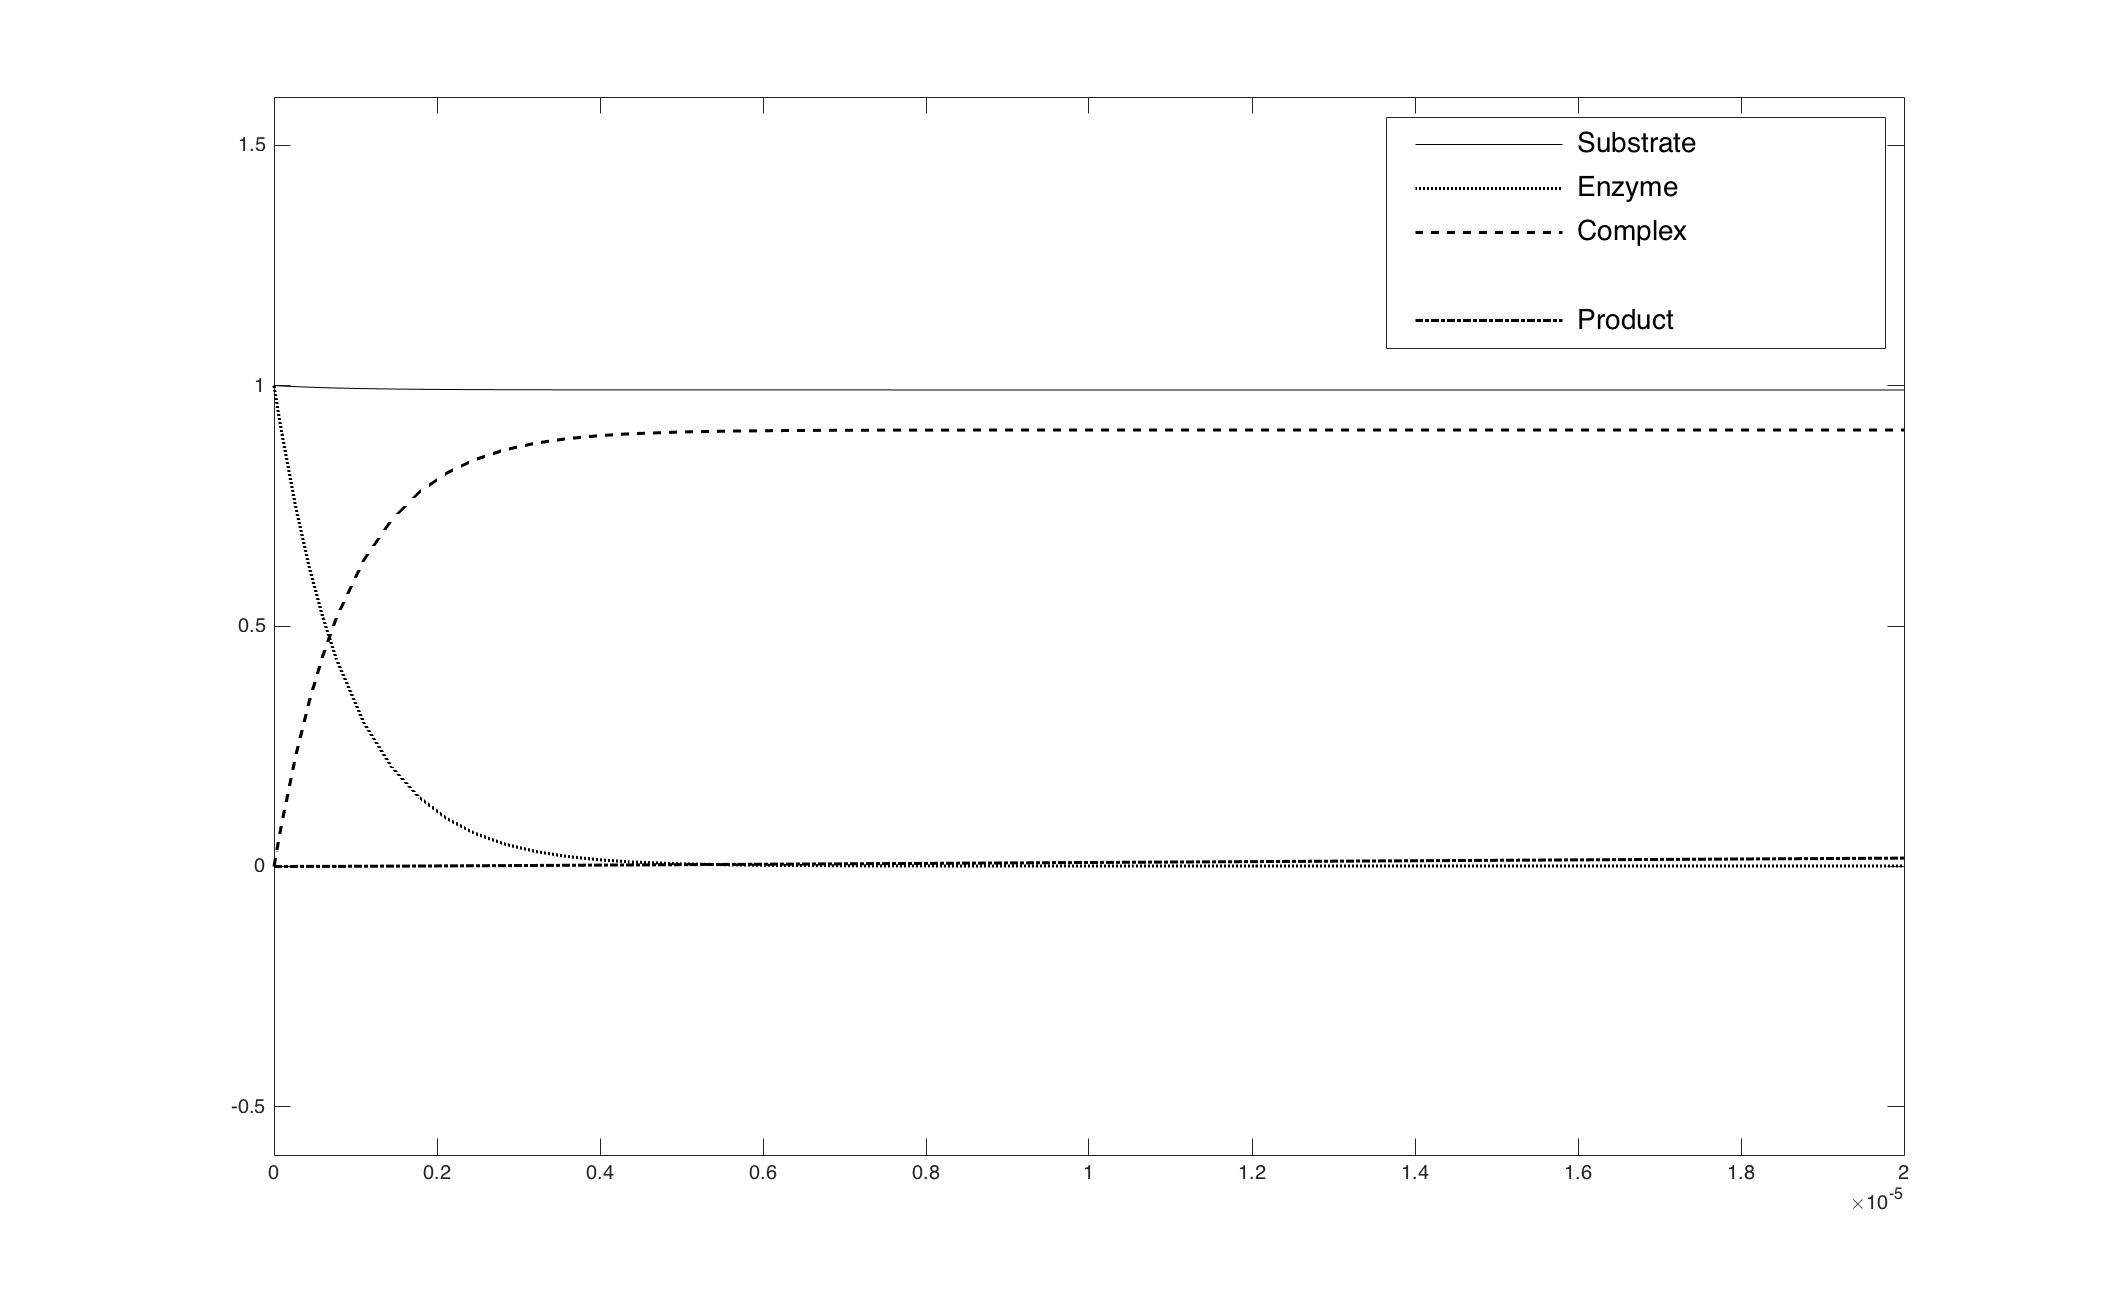
\includegraphics[width=0.75\textwidth]{MMTimeViewAll.jpg}   
   \caption{Generalized Michaelis-Menten Function Output over Time}
  \centering
\end{figure} 
%~~~~~~Figure Example~~~~~~
\begin{figure}
 \label{fig:2}[h]
    \centering
    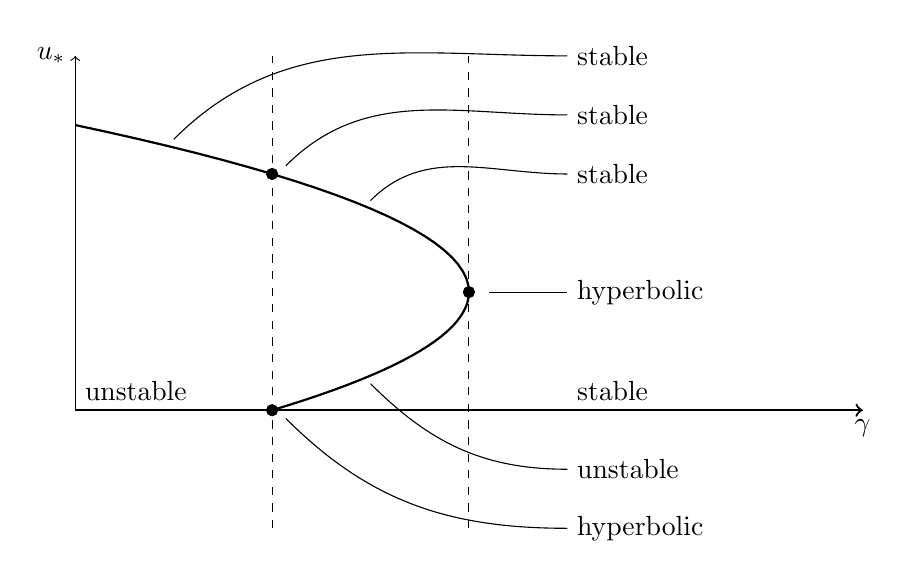
\begin{tikzpicture}[domain=0:{sqrt(2)},label/.style={
        postaction={decorate,transform shape,
          decoration={markings, mark=at position .5 with \node #1;}}},x=2.5cm,y=1.5cm]
      \draw[<-] (0,3) node [left] {$u_*$} -- (0,0) -- (4,0) node [below] {$\gamma$};

      \draw[-,thick] plot(-\x^2+2,{\x+1});
      \draw[-,thick,domain=0:1] plot(-\x^2+2,{-\x+1});
      \draw[->,thick] (0,0) -- (4,0);
      \draw (2.5,0) node[above right]{stable};

      \draw[dashed] (1,-1) -- (1,3);
      \draw[dashed] (2,-1) -- (2,3);

      \draw[fill] (1,2) circle (2pt);
      \draw[fill] (1,0) circle (2pt);
      \draw[fill] (2,1) circle (2pt);

      \draw[-] (1.5,{sqrt(1.5)-1}) to [out=-45,in=180] (2.5,-0.5)
      node[right]{unstable};
      \draw[-] (1.5,{-sqrt(1.5)+3}) to [out=45,in=180] (2.5,2)
      node[right]{stable};

      \draw[-] (1+0.07,{sqrt(1)-1-0.07}) to [out=-45,in=180] (2.5,-1)
      node[right]{hyperbolic};
      \draw[-] (1+0.07,{-sqrt(1)+3+0.07}) to [out=45,in=180] (2.5,2.5)
      node[right]{stable};

      \draw[-] (0.5,{-sqrt(0.5)+3}) to [out=45,in=180] (2.5,3)
      node[right]{stable};

      \draw[-] (2+0.1,1) -- (2.5,1) node[right]{hyperbolic};

      \draw (0,0) node[above right]{unstable};
    \end{tikzpicture}
    \caption{This is a placeholder for Our Bifurcation Diagram}
  \end{figure}
%~~~~~~Figure Example~~~~~~
% one-column
\begin{figure}
\label{fig:3}[h]
 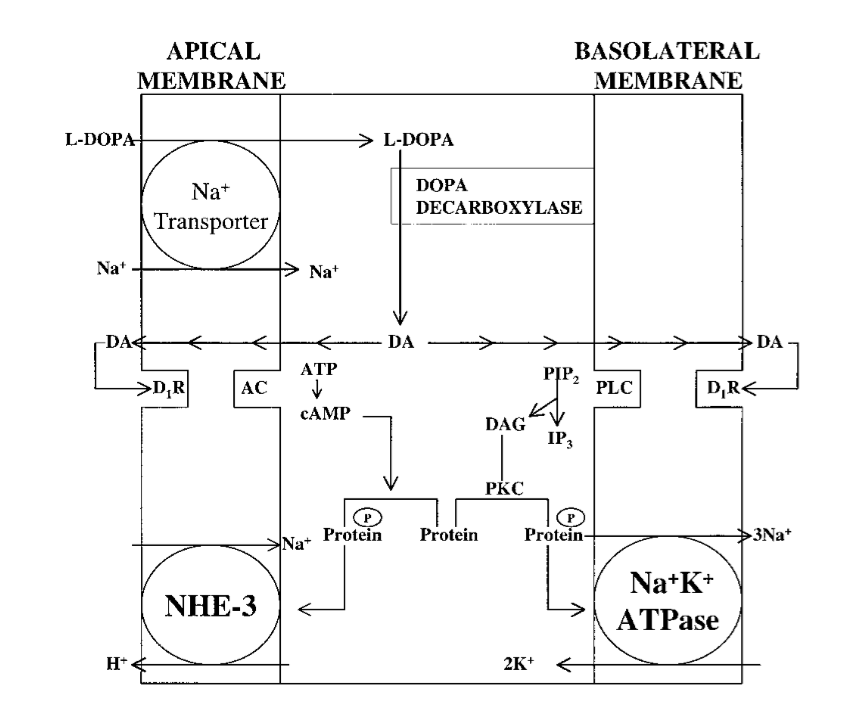
\includegraphics[width=0.75\textwidth]{Schematic_Renal_Dopamine.png}   
   \caption{Schematic depiction of dopamine formation and cell signaling mechanisms activating sodium transport across the proximal renal tubule cell \cite{Ref30}}
  \centering
\end{figure} 
%~~~~~~Figure Example~~~~~~
% one-column wide fig
%\begin{figure}[h]
%\label{fig:4}
 %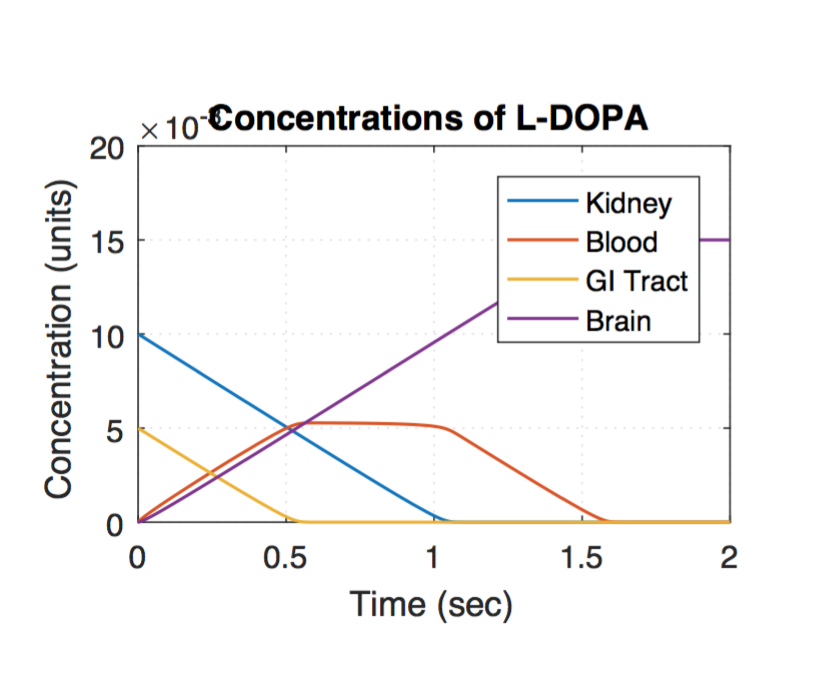
\includegraphics[width=0.75 \textwidth]{InitialSimulationGraph}   
  % \caption{Levels of L-DOPA in Each System}
 % \centering
%\end{figure}
%~~~~~~Figure Example~~~~~~
%% For one-column wide figures use
%\begin{figure}
% Use the relevant command to insert your figure file.
% For example, with the graphicx package use
 % 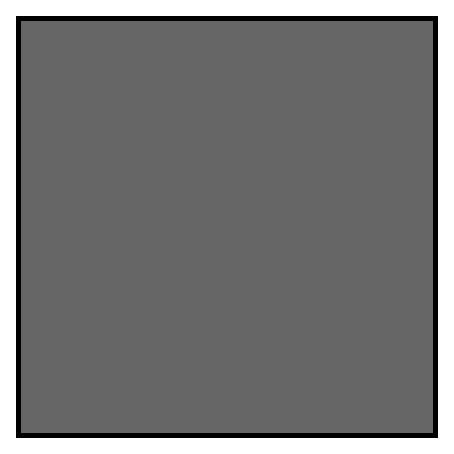
\includegraphics{example.eps}
% figure caption is below the figure
%\caption{Please write your figure caption here}
%\label{fig:1}       % Give a unique label
%\end{figure}
%~~~~~~Figure Example~~~~~~
% For two-column wide figures use
%\begin{figure*}
% Use the relevant command to insert your figure file.

%  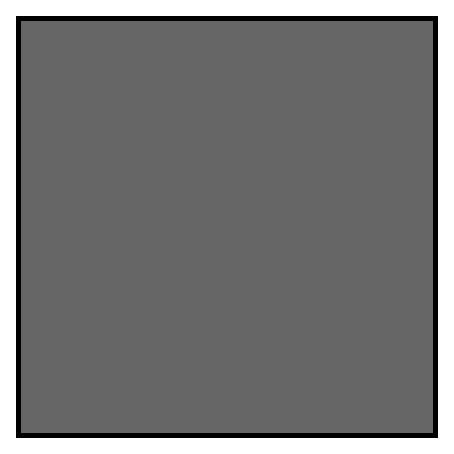
\includegraphics[width=0.75\textwidth]{example.eps}
% figure caption is below the figure
%\caption{Please write your figure caption here}
%\label{fig:2}      
%\end{figure*}

%~~~~~ Table Example~~~~~~
%\begin{table}
% table caption is above the table
%\caption{Please write your table caption here}
%\label{tab:1}       
% For LaTeX tables use
%\begin{tabular}{lll}
%\hline\noalign{\smallskip}
%first & second & third  \\
%\noalign{\smallskip}\hline\noalign{\smallskip}
%number & number & number \\
%number & number & number \\
%\noalign{\smallskip}\hline
%\end{tabular}
%\end{table}
%~~~~~~Figure Example~~~~~~
%\begin{figure}                                       
%\label{fig:2}
% 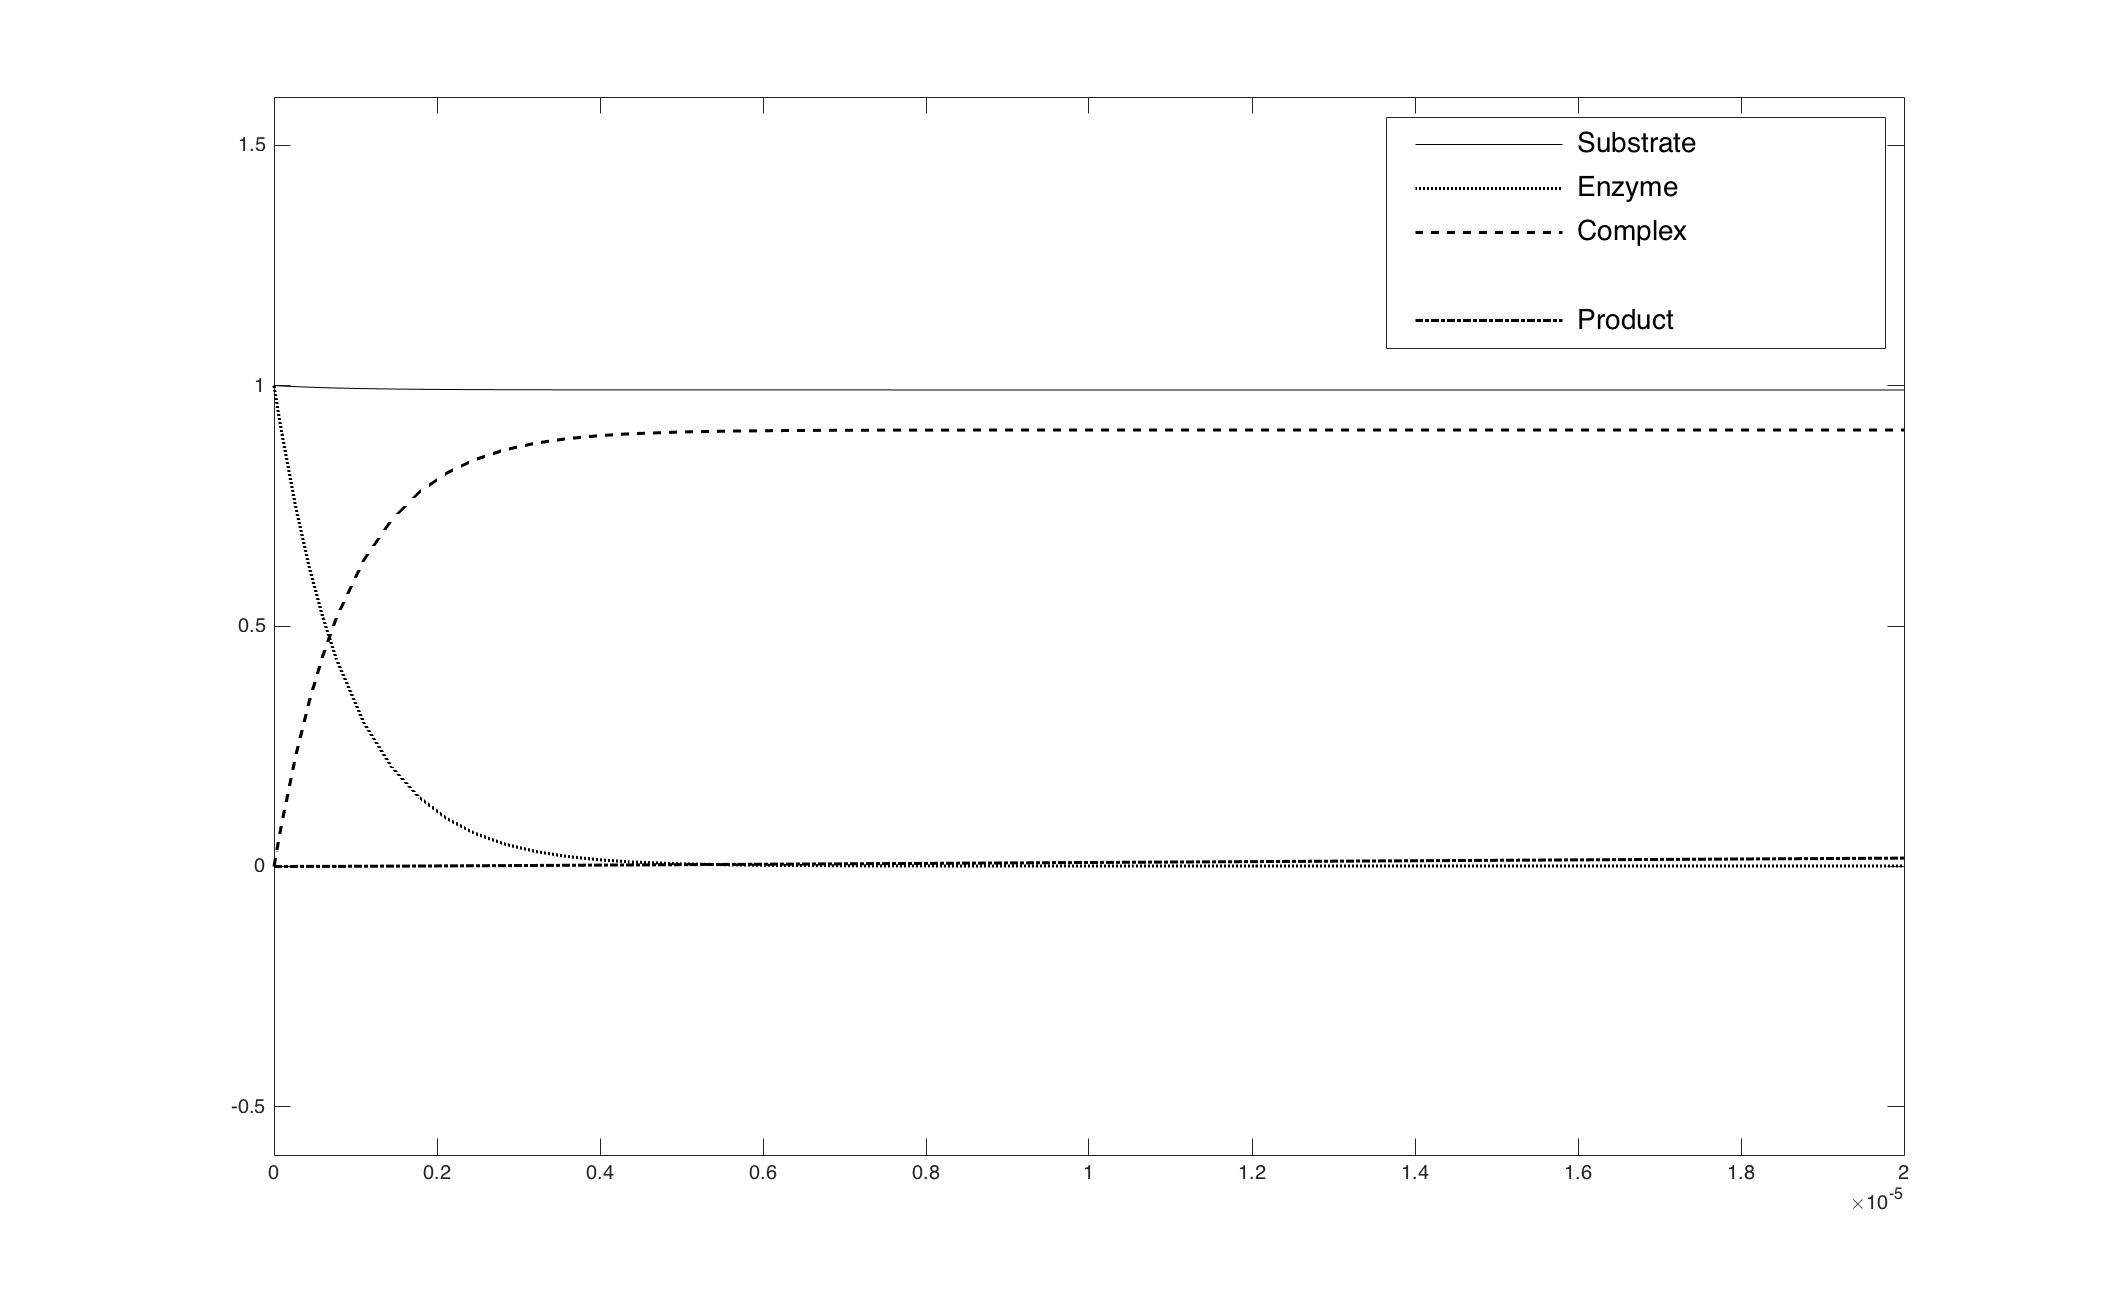
\includegraphics[width=0.75\textwidth]{MMTimeViewAll.jpg}  
%   \caption{Please write your figure caption here}
%\end{figure}                                     
%~~~~~~Figure Example~~~~~~
% two-column wide figures
%\begin{figure}[h]                                 
%\label{fig:5}
%  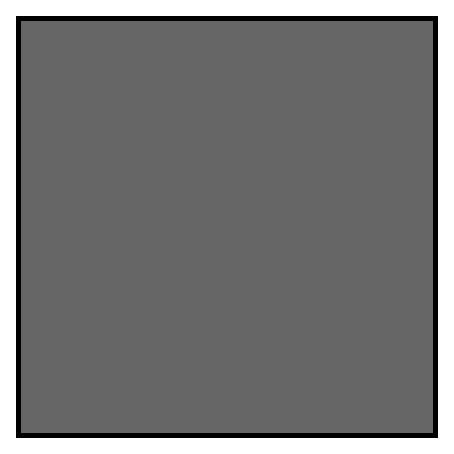
\includegraphics[width=0.75\textwidth]{example.eps}
%\caption{Please write your figure caption here}
%\end{figure}
%
%\subsection{Tables}
%~~~~~~Table 1 ~~~~~
\begin{table}[h]
\caption{Michaelis Menten Rates}         
\label{tab:1}                                         
\begin{tabularx}{\textwidth}{XXXXX}      
\hline\noalign{\smallskip}
Variable Name & Value & Description & Unit & Dimensions \\
\noalign{\smallskip}\hline\noalign{\smallskip}
$N_A$      & $6.022 \times 10^23$ & Avogadro Constant     & $mol^{-1}$                      &N \\
$c$        & --                  & molarity               & $\frac{N}{(N_A \cdot V)}$       & $\frac{[n]}{V}$\\
$\alpha_1$ & 3.0                 & molarity/time          & $\frac{C_i}{s}$          & $\frac{[n]}{V \cdot t}$\\    
$\alpha_2$ & 2.0                 & molarity/time          & $\frac{C_i}{s}$          & $\frac{[n]}{V \cdot t}$ \\     
$\alpha_3$ & --                  & molarity/time          & $\frac{C_i}{s}$          & $\frac{[n]}{V \cdot t}$ \\
$\alpha_4$ & --                  & molarity/time          & $\frac{C_i}{s}$          & $\frac{[n]}{V \cdot t}$ \\
$\alpha_5$ & --                  & molarity/time          & $\frac{C_i}{s}$          & $\frac{[n]}{V \cdot t}$ \\
$\alpha_6$ & --                  & molarity/time          & $\frac{C_i}{s}$          & $\frac{[n]}{V \cdot t}$ \\
$\alpha_7$ & --                  & molarity/time          & $\frac{C_i}{s}$          & $\frac{[n]}{V \cdot t}$ \\
$\alpha_8$ & --                  & molarity/time          & $\frac{C_i}{s}$          & $\frac{[n]}{V \cdot t}$ \\
\noalign{\smallskip}\hline
\end{tabularx}
\end{table}
%~~~~~~ Table 2 ~~~~~~
%\begin{table}[h]
%\caption{This Table is a Place Holder}
%\label{tab:2}
%\begin{tabularx}{\textwidth}{XXXXX}
%\hline\noalign{\smallskip}
%-- & -- & -- & -- & -- \\
%\noalign{\smallskip}\hline\noalign{\smallskip}
%$--$ & -- & -- & -- & -- \\
%$--$ & -- & -- & -- & -- \\
%$--$ & -- & -- & -- & -- \\
%$--$ & -- & -- & -- & -- \\
%$--$ & -- & -- & -- & -- \\
%$--$ & -- & -- & -- & -- \\
%$--$ & -- & -- & -- & -- \\
%$--$ & -- & -- & -- & -- \\
%$--$ & -- & -- & -- & -- \\
%$--$ & -- & -- & -- & -- \\
%$--$ & -- & -- & -- & -- \\
%$--$ & -- & -- & -- & -- \\
%$--$ & -- & -- & -- & -- \\
%\end{tabularx}
%\end{table}
%~~~~~~Acknowledgments~~~~~~
\section{Acknowledgments and Works Cited}
\label{sec:10}
%~~~~~~Acknowledgments~~~~~~
\subsection{Acknowledgments}
\todo{Write Acknowledgments} 
\begin{acknowledgements}
\end{acknowledgements}

%~~~~~~Bibliography~~~~~~
\subsection{Works Cited and Works Consulted}
\bibliographystyle{spmpsci}                      
\begin{thebibliography}{}
\bibitem{Ref1}
D.L. Penry, P.A. Jumars, Ecology of Marine Deposit Feeders: Digestion Theory Applied to Deposit Feeding, pp 114-128 (1989)
\bibitem{Ref2}
, Book title, page numbers. Publisher, place (year); 
\bibitem{Ref3} 
Caltech Tables
\bibitem{Ref4}
\bibitem{Ref5}
\bibitem{Ref6}
    2015 Elsevier Inc. Published by Elsevier Inc. 
Received: September 25, 2014; Received in revised form: December 16, 2014; Accepted: February 18, 2015; Published April 9, 2015
\bibitem{Ref7}
Wolesensky, William; Logan, David; Grasshopper Digestion Paper; (2005) 
\bibitem{Ref8}
By User:Slashme; Patrick J. Lynch; User:Fvasconcellos - self-made; re-use File:Brain bulbar region.svg, GFDL, https://commons.wikimedia.org/w/index.php?curid=44402772
\bibitem{Ref9}
    Malenka RC, Nestler EJ, Hyman SE (2009). "Chapter 6: Widely Projecting Systems: Monoamines, Acetylcholine, and Orexin". In Sydor A, Brown RY. Molecular Neuropharmacology: A Foundation for Clinical Neuroscience (2nd ed.). New York: McGraw-Hill Medical. pp. 147–148, 154–157. ISBN 9780071481274.
\bibitem{Ref10}
   Malenka RC, Nestler EJ, Hyman SE (2009). "Chapter 10: Neural and Neuroendocrine Control of the Internal Milieu". In Sydor A, Brown RY. Molecular Neuropharmacology: A Foundation for Clinical Neuroscience (2nd ed.). New York: McGraw-Hill Medical. p. 249. ISBN 9780071481274.
\bibitem{Ref11}
Le Moal, Michel. "Mesocorticolimbic Dopaminergic Neurons". Neuropsychopharmacology: The Fifth Generation of Progress. Retrieved 4 November 2013
\bibitem{Ref12}
Rang, H. P. (2003). Pharmacology. Edinburgh: Churchill Livingstone. pp. 474 for noradrenaline system, page 476 for dopamine system, page 480 for serotonin system and page 483 for cholinergic system. ISBN 0-443-07145-4.
\bibitem{Ref13}
By Thomas Splettstoesser (www.scistyle.com) - Own work, CC BY-SA 4.0, https://commons.wikimedia.org/w/index.php?curid=41349083
\bibitem{Ref14}
Kolb, Bryan; Whishaw, Ian Q. (2003). Fundamentals of Human Neuropsychology (5th ed.). Worth. pp. 102–104. ISBN 978-0-7167-5300-1. (reference for all five stages)
\bibitem{Ref15}
http://www.uptodate.com/contents/renal-actions-of-dopamine/abstract/1-3?utdPopup=true
\bibitem{Ref16}
Carey RM, Theodore Cooper Memorial Lecture: Renal Dopamine System Paracrine Regulator of Sodium Homeostasis and Blood Pressure. AHA Journals. doi: 10.1161/hy0901.096422
\bibitem{Ref17}
By Fvasconcellos 02:58, 14 August 2007 (UTC) - From PDB entry 1JS3. More information:Burkhard P, Dominici P, Borri-Voltattorni C, Jansonius JN, Malashkevich VN (2001). "Structural insight into Parkinson's disease treatment from drug-inhibited DOPA decarboxylase". Nat Struct Biol 8 (11): 963–7. PMID 11685243. doi:10.1038/nsb1101-963, Public Domain
\bibitem{Ref18}
Gonzales; Lecture Notes and Materials (2016)
\bibitem{Ref19}
Gerard DS Showing Protein Aromatic-L-amino-acid decarboxylase (HMDBP00278). In: Human Metabolome Database: http://www.hmdb.ca/proteins/hmdbp00278. Accessed 29 Jun 2016
\bibitem{Ref20}
Sadun; Applied Linear Algebra: The Decoupling Process (2016)      %Markov
\bibitem{Ref21}
\bibitem{Ref22}
\bibitem{Ref23}
\bibitem{Ref24}
\bibitem{Ref25}
\bibitem{Ref26}
https://github.com/hershal/m374m/blob/master/homeworks/hw3/hw3.tex
\bibitem{Ref27} 
LaTex Template: Original by Springer Heidelberg, 2010/09/16
\bibitem{Ref28}
Logan, J. David; Applied Mathematics 4th. ed. Online, pg 225     %Menten
\bibitem{Ref29}
Holzbecher, Ekkehard; Environmental Modeling                     %Menten
\bibitem{Ref30}
O’Connell DP, Ragsdale NV, Boyd DG, Felder RA, Carey RM. Differential human renal tubular responses to dopamine type 1 receptor stimulation are determine by blood pressure status. Hypertension. 1997; 29: 115–122.
\bibitem{Ref31}
http://www.lifeextension.com/Protocols/Neurological/Parkinsons-Disease/
\bibitem{Ref32}
Goldberg LI. Cardiovascular and renal actions of dopamine: potential clinical applications. Pharmacol Rev. 1972;24:1–29.
\bibitem{Ref33}
The National Collaborating Centre for Chronic Conditions, ed. (2006). "Symptomatic pharmacological therapy in Parkinson’s disease". Parkinson's Disease. London: Royal College of Physicians. pp. 59–100. ISBN 1-86016-283-5. Retrieved 10 June 2016
\bibitem{Ref34}
http://www.cell.com/trends/neurosciences/pdf/S0166-2236(07)00051-3.pdf
\bibitem{Ref35}
Jupyter and Github Links
\bibitem{Ref36}
http://arbl.cvmbs.colostate.edu/hbooks/molecules/cyclase.html
%
\bibitem{RefJ}
Author, Article title, Journal, Volume, page numbers (year)
\bibitem{RefB}
Author, Book title, page numbers. Publisher, place (year)
\end{thebibliography}
\end{document}
% end of file template.tex